\newprob{qone}{
\adjustbox{valign=t,center}{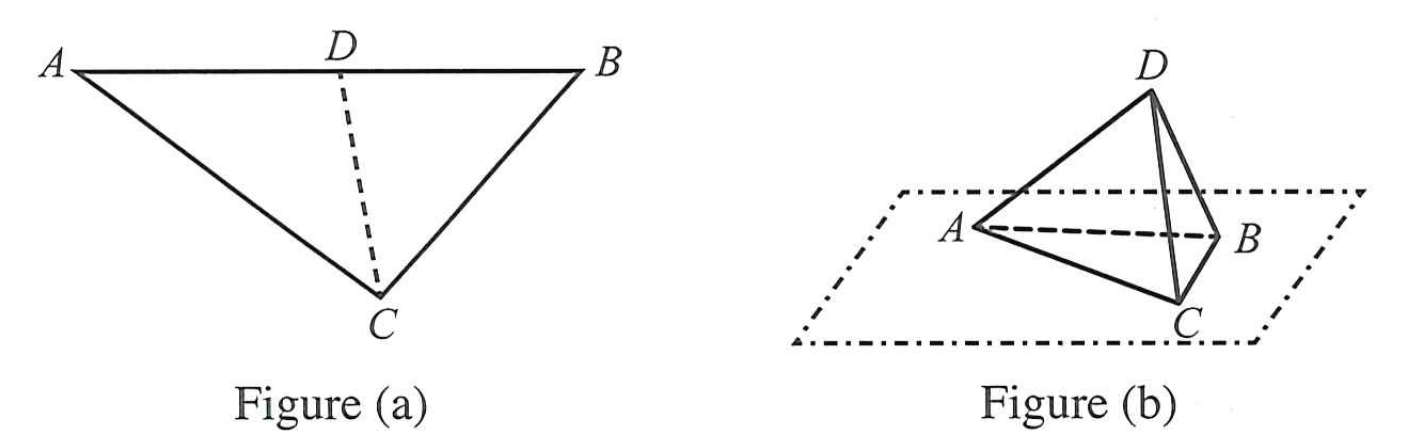
\includegraphics[width=0.75\linewidth]{assets/adad.png}}
\begin{parts}
    \part Figure (a) shows a piece of triangular paper card $ABC$ with $AB$ = 40 cm, $BC$ = 24 cm and $AC$ = 30 cm. Let $D$ be a point lying on $AB$ such that $\angle$$BDC$ = \dg{80}.
    \begin{subparts}
        \subpart Find $\angle$$DBC$.
        \subpart Find the length of $AD$.
    \end{subparts}\zh{4}
    \part The triangular paper card described in (a) is folded along $CD$ such that $AC$ and $BC$ lie on the horizontal ground as shown in Figure (b). It is given that $\angle$$ADB$ = \dg{64}.
    \begin{subparts}
        \subpart Find the distance between $A$ and $B$ on the horizontal ground.
        \subpart Let $M$ be a point lying on $BC$ such that $DM$ is perpendicular to $BC$. Someone claims that the angle between the face $DBC$ and the horizontal ground is $\angle$$DMA$. Do you agree? Explain your answer.
    \end{subparts}\zh{5}

\end{parts}
}{
    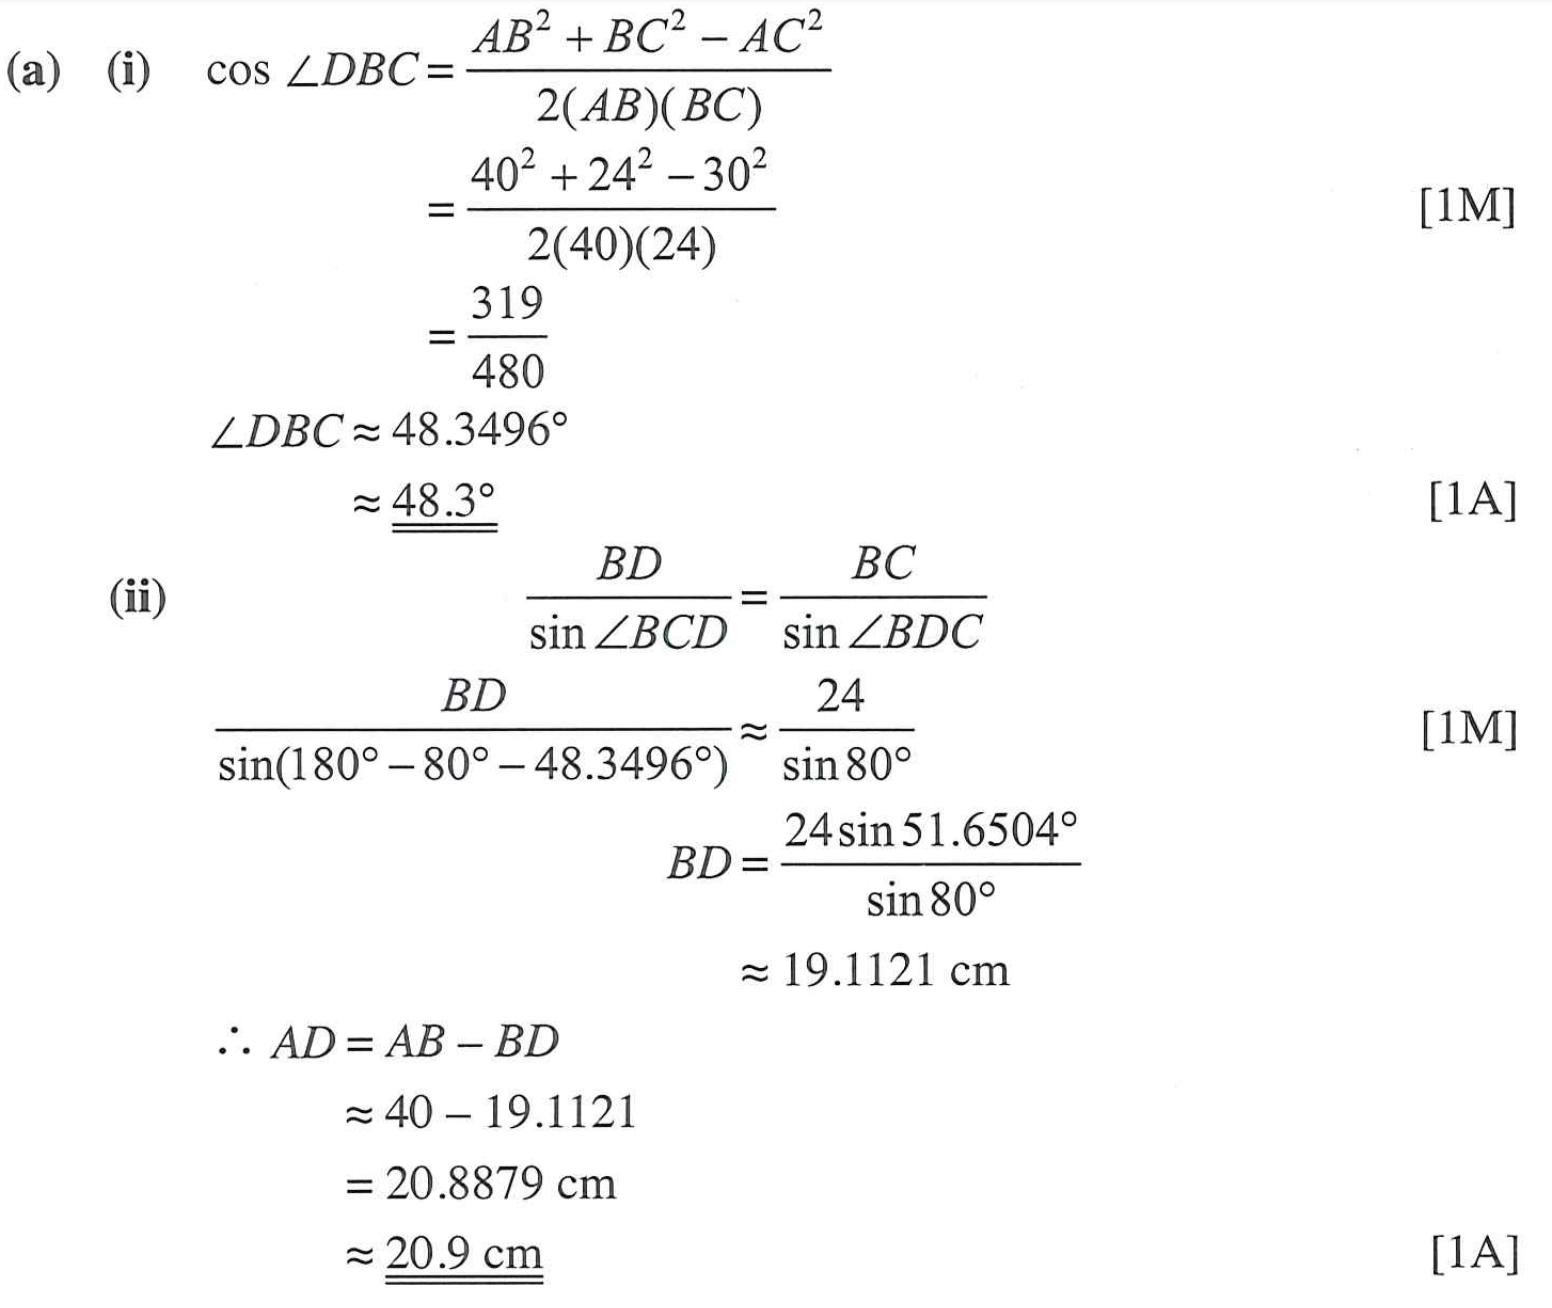
\includegraphics[width=0.75\linewidth]{assets/jdoi2.png}
    \par 
    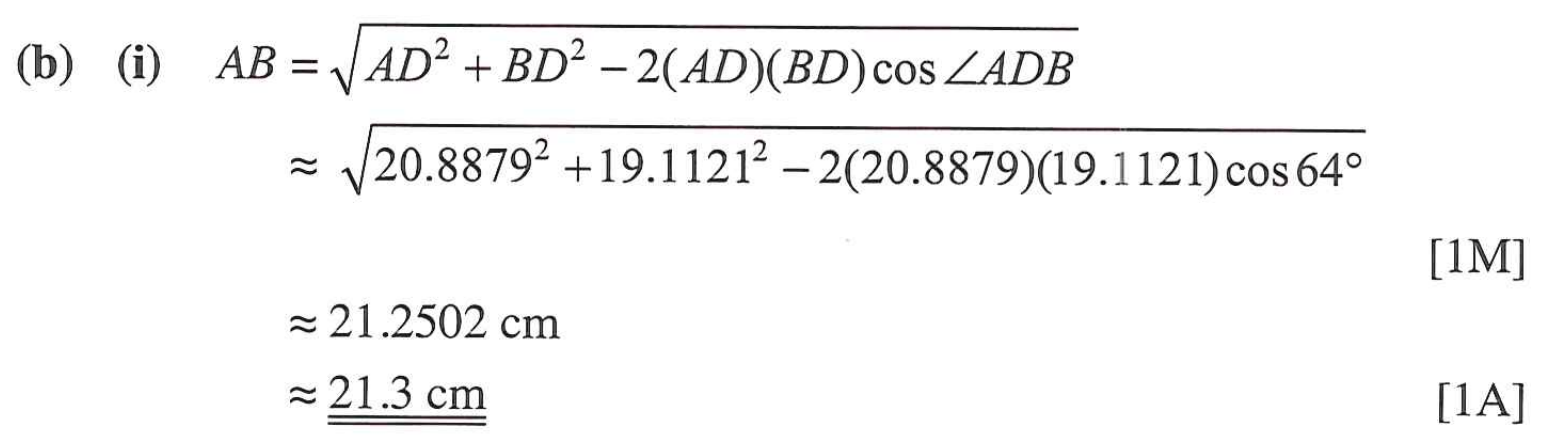
\includegraphics[width=0.75\linewidth]{assets/doiipdj.png}
    \par 
    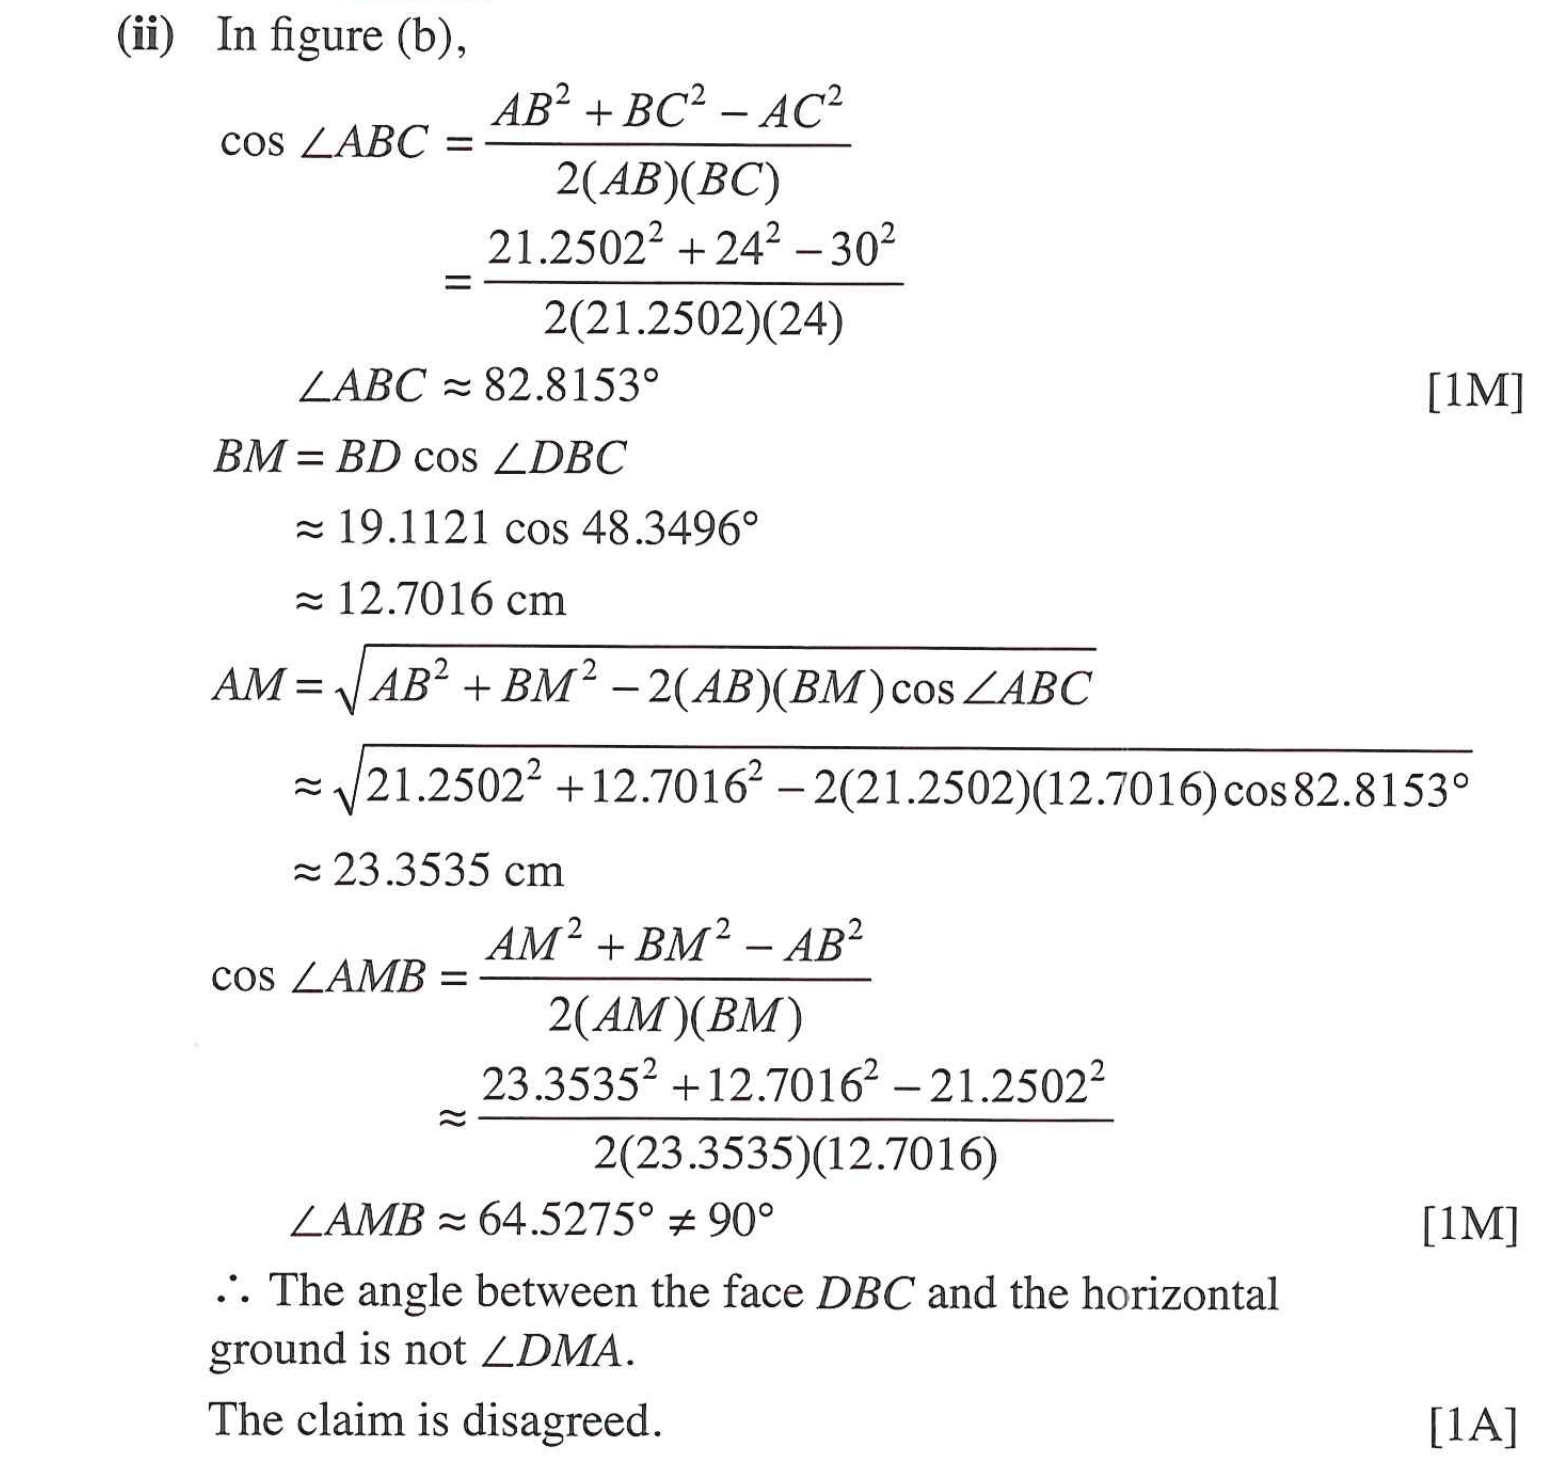
\includegraphics[width=0.75\linewidth]{assets/dqdwqd13.png}
}

\newprob{qtwo}{
    \topalignc{
    
    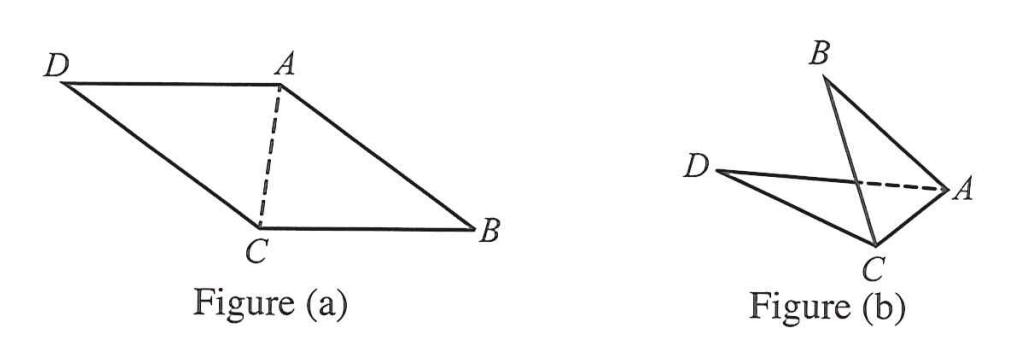
\includegraphics[width=0.75\linewidth]{assets/ddwd2f.png}
    }
    \begin{parts}
        \part In Figure (a), $ABCD$ is a paper card in the shape of a parallelogram. It is given that $AB$ = 24 cm, $\angle$$ABC$ = \dg{36} and $\angle$$BAC$ = \dg{62}. Find the length of $BC$. \zh{2}
        \part The paper card in Figure (a) is folded along $AC$ such that the distance between $B$ and $D$ is 16 cm (see Figure (b)).
        \begin{subparts}
            \subpart Find $\angle BCD$.
            \subpart Find the angle between the plane $ABC$ and the plane $ADC$.
        \end{subparts}
    \end{parts}
    
}{
    {\par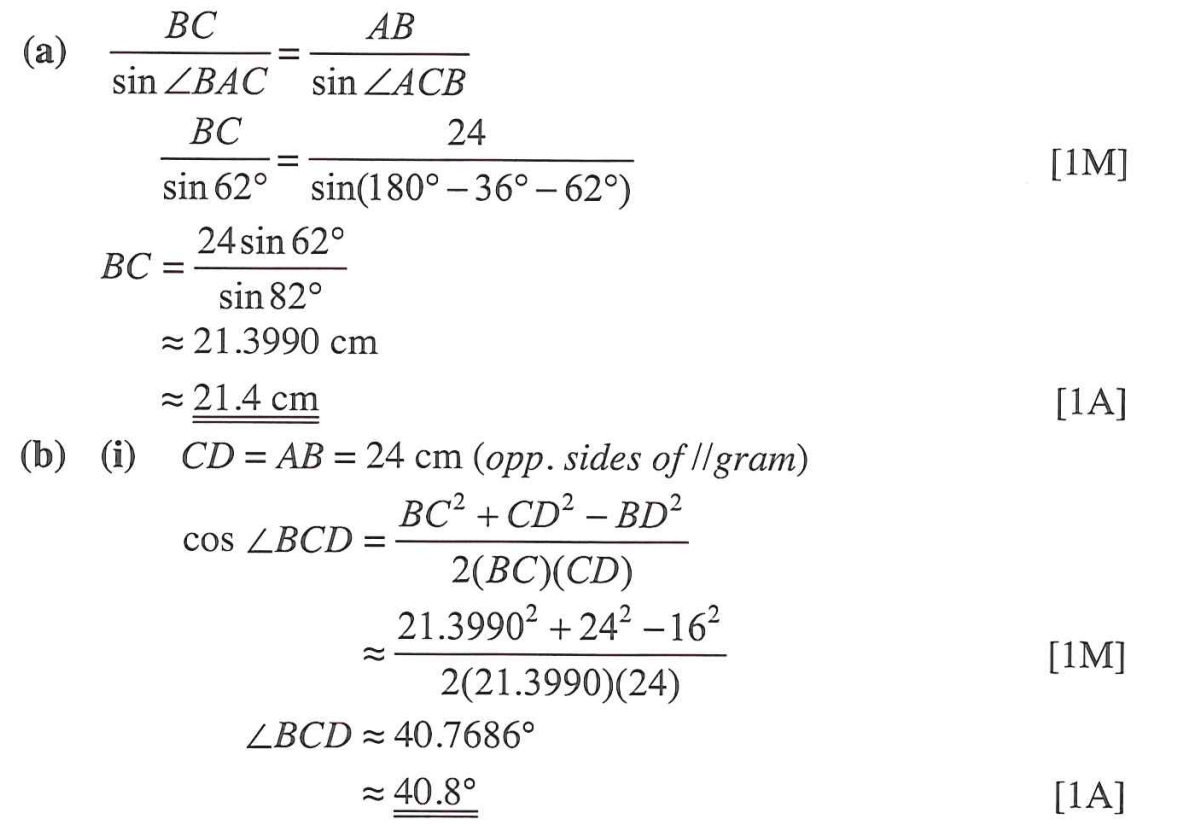
\includegraphics[width=0.75\linewidth]{assets/huiewfciqweuh.png}\par}
    {\par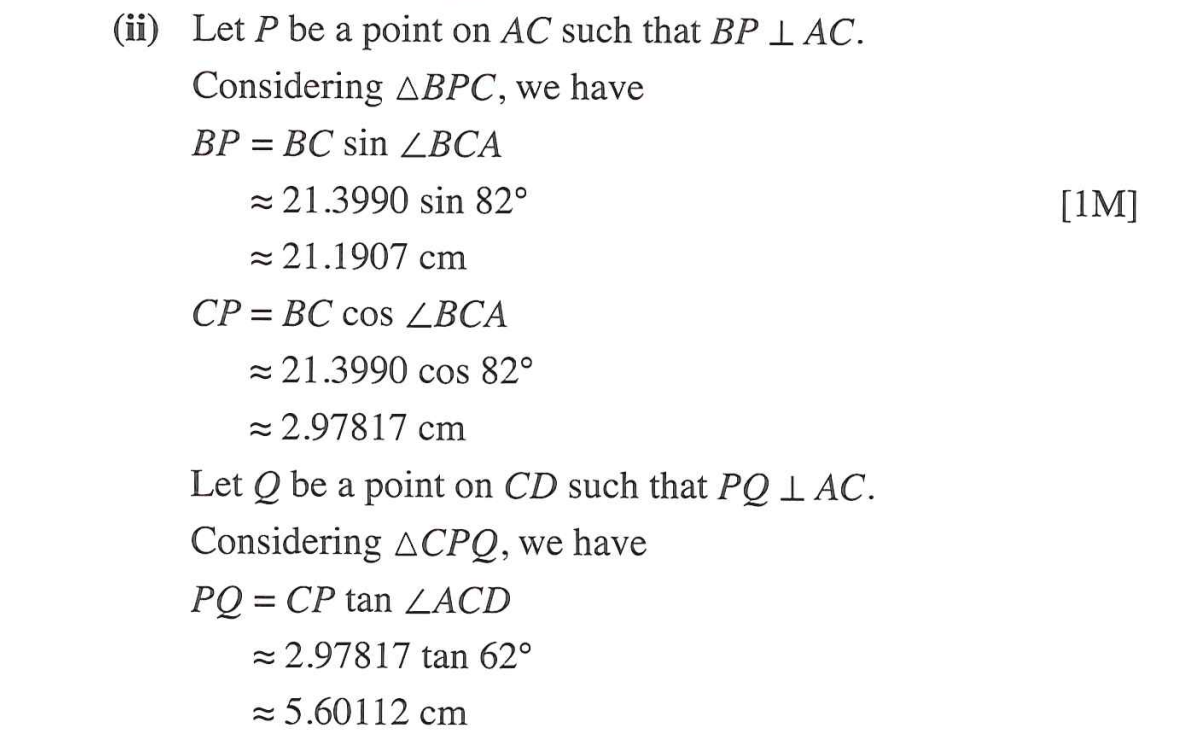
\includegraphics[width=0.75\linewidth]{assets/ddiwdjowqdwqidjoiwqjdoiwqw.png}\par}
    {\par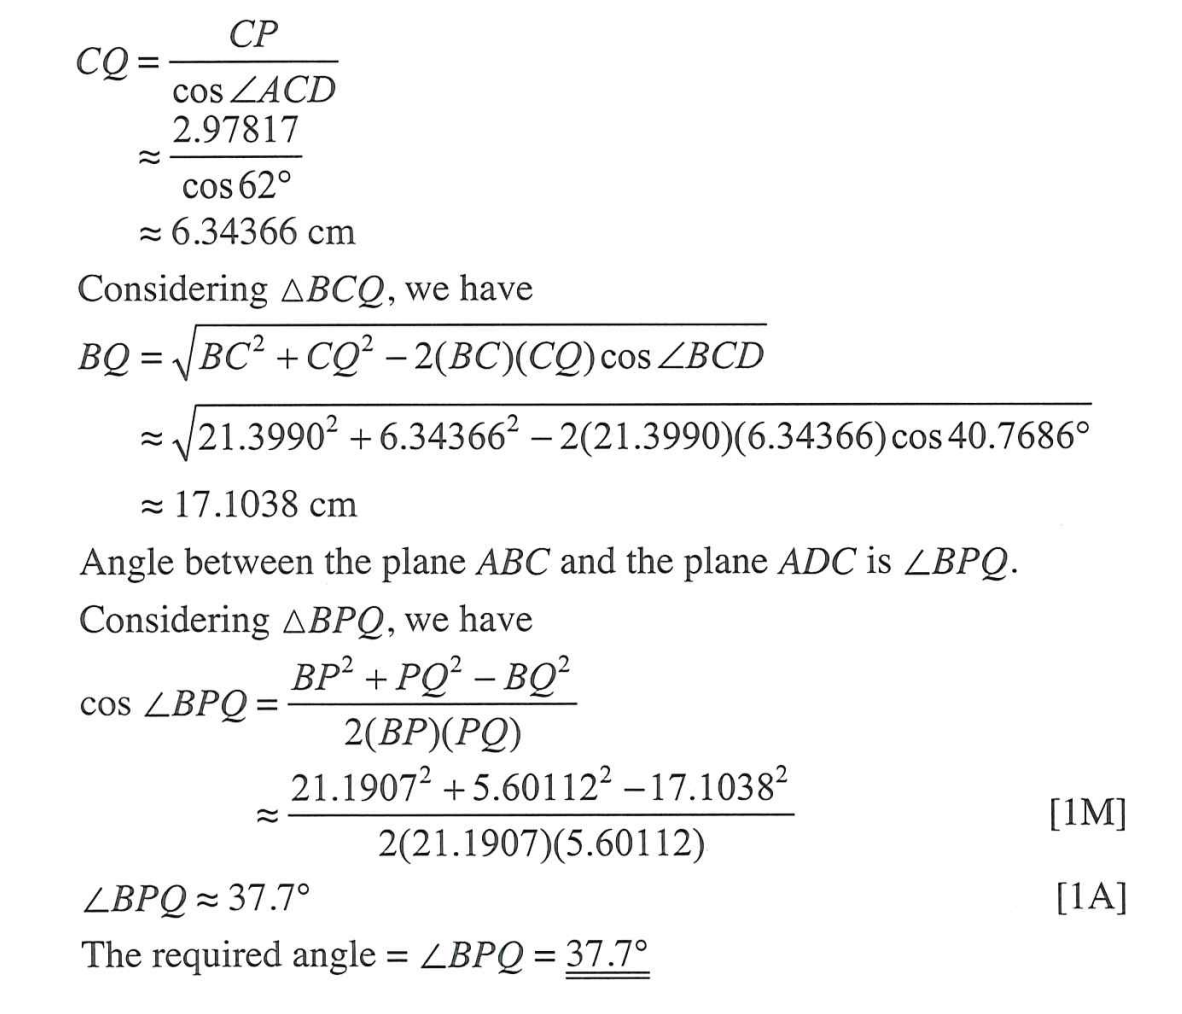
\includegraphics[width=0.75\linewidth]{assets/adepkdoekodewpdkopwed.png}\par}
    
    
    
    
}

\newprob{qthree}{
    \topalignc{\par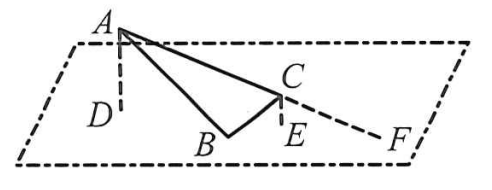
\includegraphics[width=0.4\linewidth]{assets/djiewdioewjdpwei8.png}}
    $ABC$ is a thin triangular metal sheet, where $BC$ = 20 cm, $\angle BAC$ = \dg{35} and $\angle ACB$ = \dg{40}.
    \begin{parts}
        \part Find the length of AC.\zh{2}
        \part In the figure, the thin metal sheet ABC is held such that only vertex B lies on the horizontal ground. D and E are points lying on the horizontal ground vertically below the vertices A and C respectively. AC produced meets the horizontal ground at the point F. A craftsman finds that AD = 9 cm and CE = 3 cm.
        \begin{subparts}
            \subpart Find the distance between C and F.
            \subpart Find the area of $\Delta$ABF.
            \subpart Find the inclination of the thin metal sheet ABC to the horizontal ground.
            \subpart The craftsman claims that the area of $\Delta$BDF is greater than 290 cm$^2$. Do you agree? Explain your answer.

        \end{subparts}\zh{11}
    \end{parts}
}
{
    {\par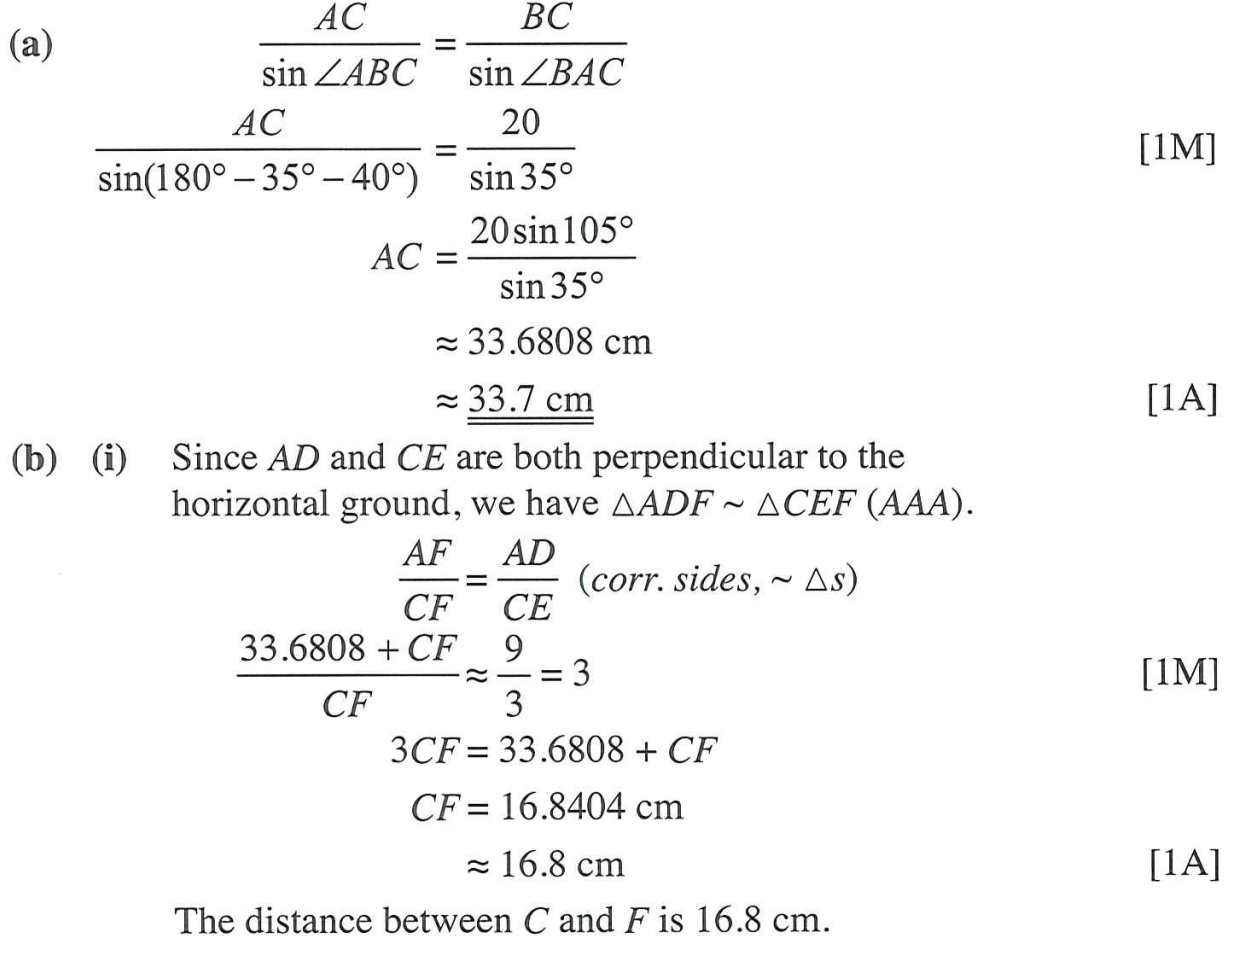
\includegraphics[width=0.75\linewidth]{assets/jiodjwqdowqjdoiqwdage.png}
    \par}
    {\par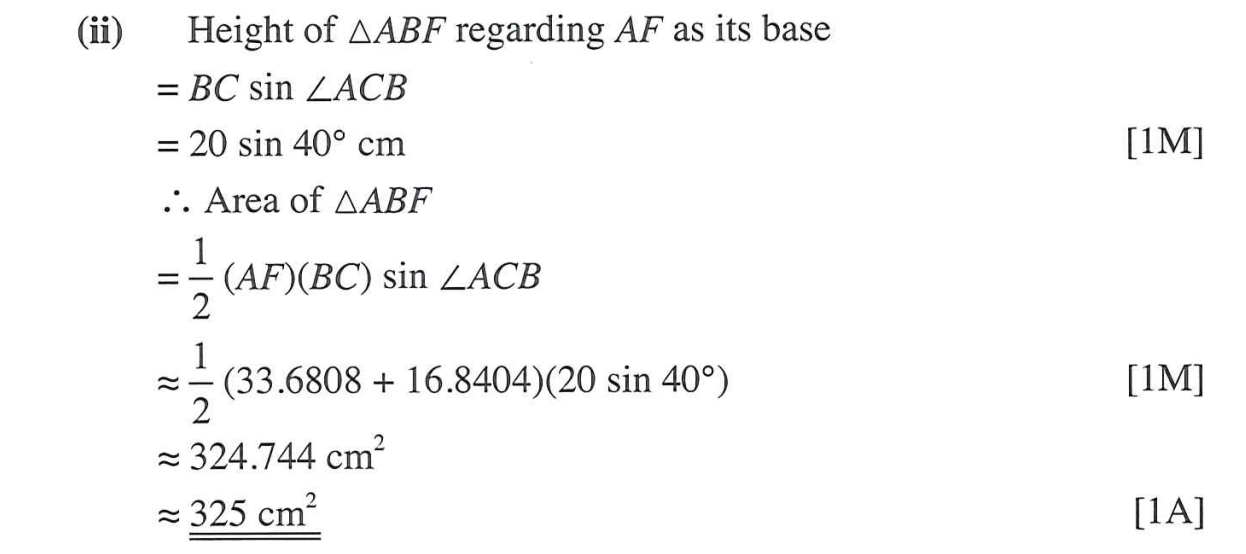
\includegraphics[width=0.75\linewidth]{assets/dijodoiqwdiowqage.png}\par}
    {\par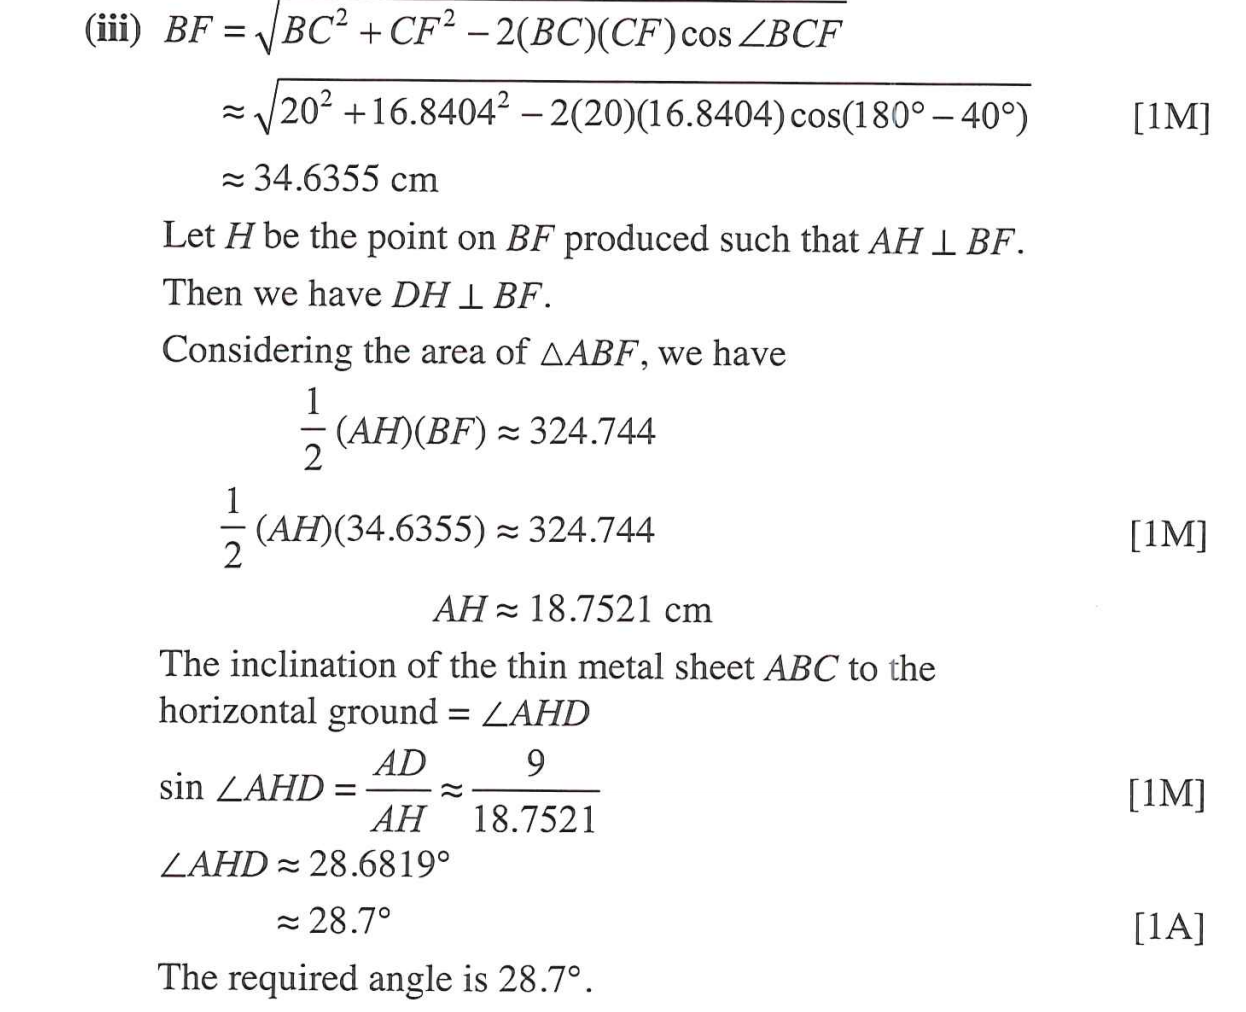
\includegraphics[width=0.75\linewidth]{assets/djdiodwjdiq.png}\par}
    {\par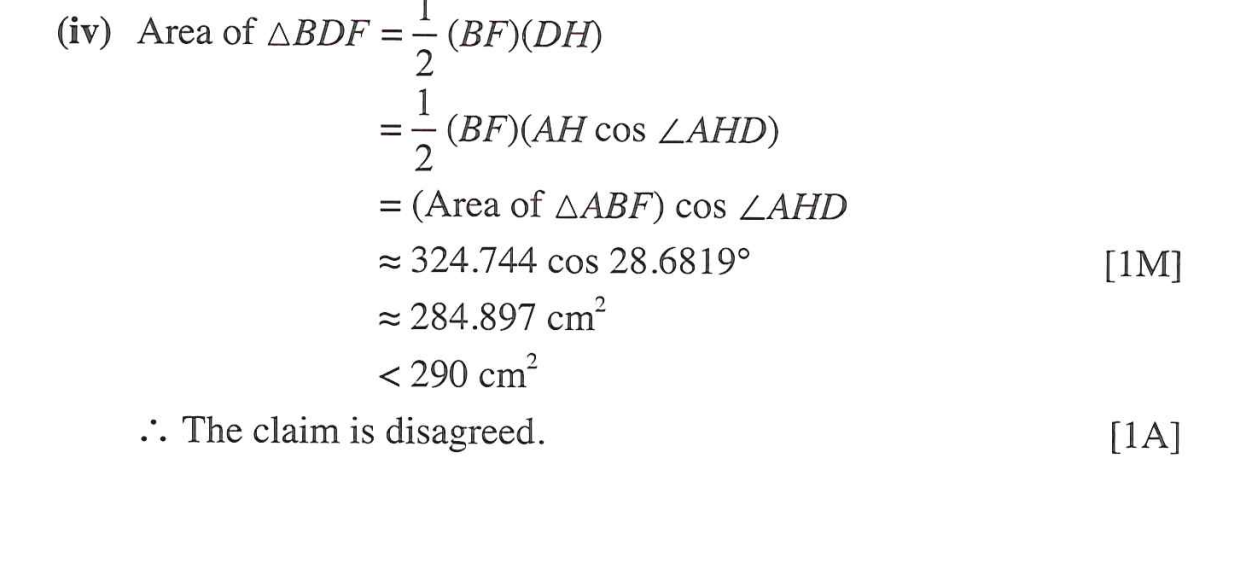
\includegraphics[width=0.75\linewidth]{assets/ddojwqodjqw.png}\par}
}

\newprob{qfour}{
    Figure (a) shows a solid pyramid VABCD with a rectangular base, where AB = 20 cm, BC = 12 cm, VB = VC = 40 cm and $\angle$VAB = $\angle$VDC = \dg{120}.{\par\centering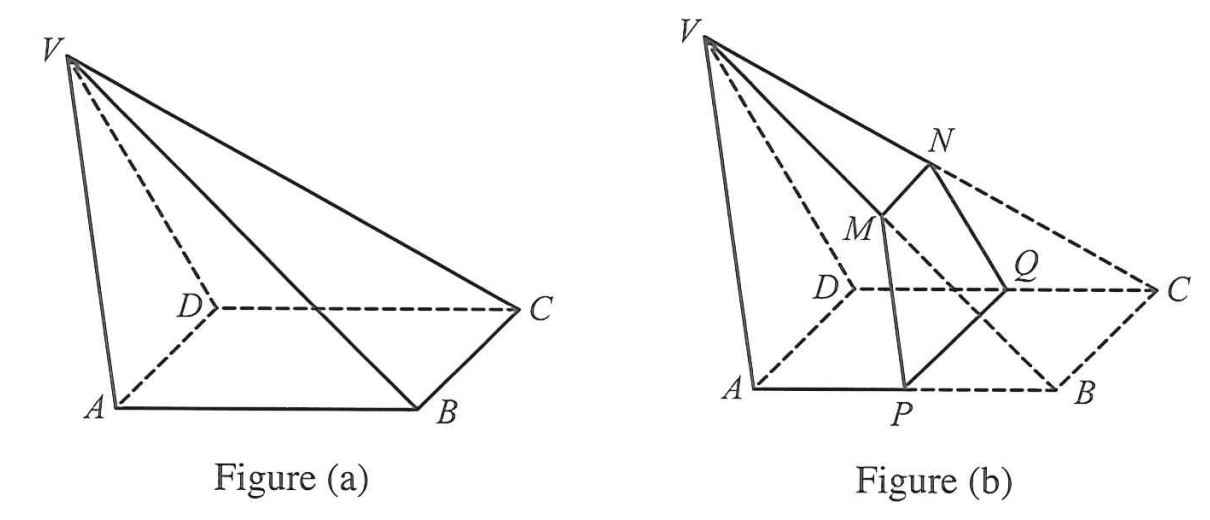
\includegraphics[width=0.75\linewidth]{assets/ddjoiqwdwijdw.png}\par}
    \begin{parts}
        \part Find $\angle VBA$.\zh{2}
        \part P, Q, M and N are the mid-points of AB, CD, VB and VC respectively. A geometric model is made by cutting off PBCQNM from VABCD as shown in Figure (b). A craftsman claims that the area of the trapezium PQNM is less than 120 cm$^2$. Do you agree? Explain your answer. \zh{5}
    \end{parts}
    
}
{
    {\par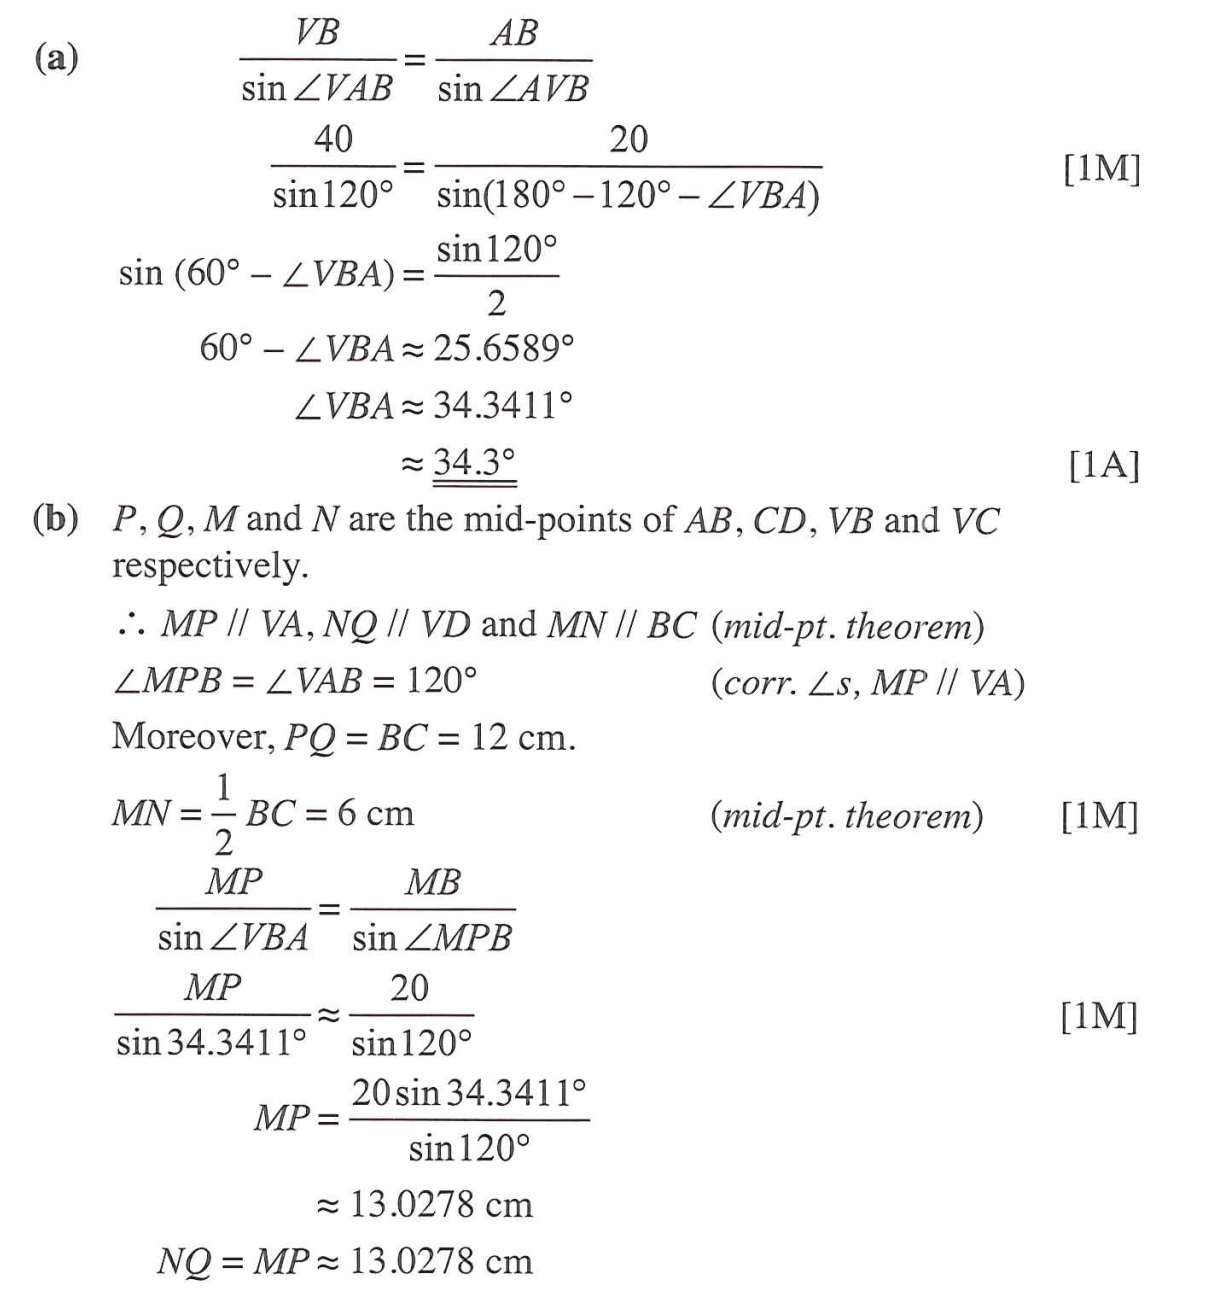
\includegraphics[width=0.75\linewidth]{assets/joaidjoajdoa.png}\par}
        {\par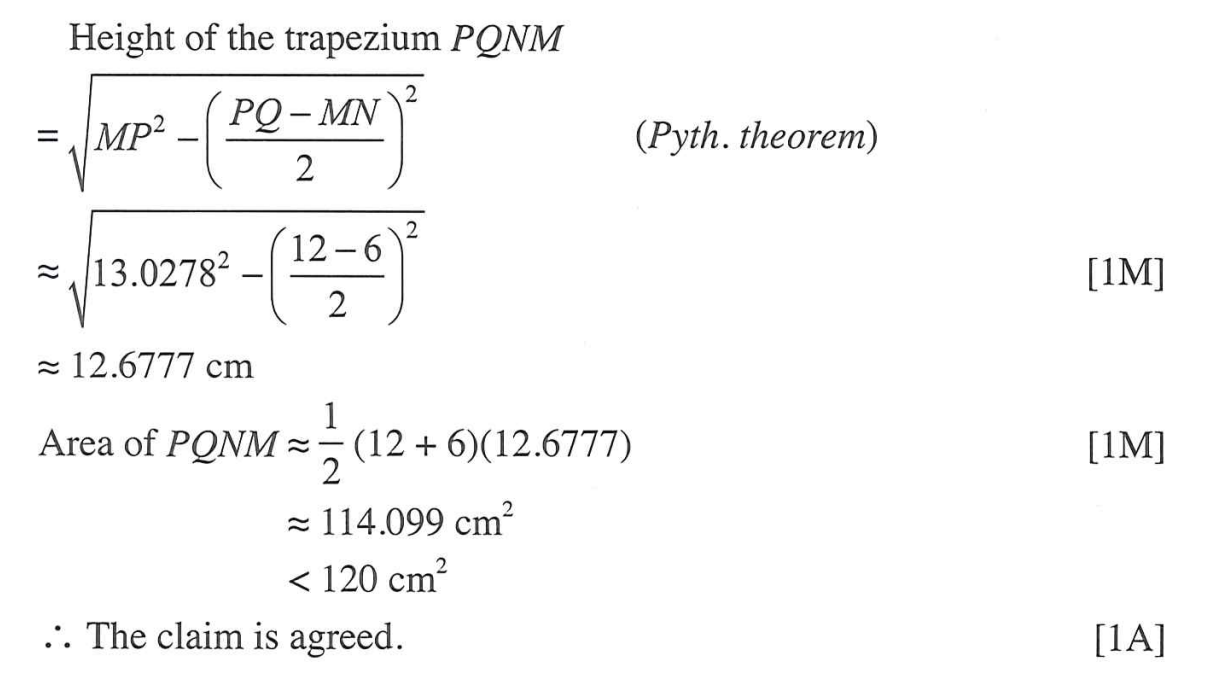
\includegraphics[width=0.75\linewidth]{assets/ddoijwqjdowiqjdoiwjqe.png}\par}
}

\newprob{qfive}{
    Figure (a) shows a right pyramid VABCD with a square base, where $\angle$VAB = \dg{70}. The length of a side of the base is 30 cm. Let P and Q be the points lying on VA and VD respectively such that PQ is parallel to BC and $\angle$PBA = \dg{50}. A geometric model is made by cutting off the pyramid VPBCQ from VABCD as shown in Figure (b).{\par\centering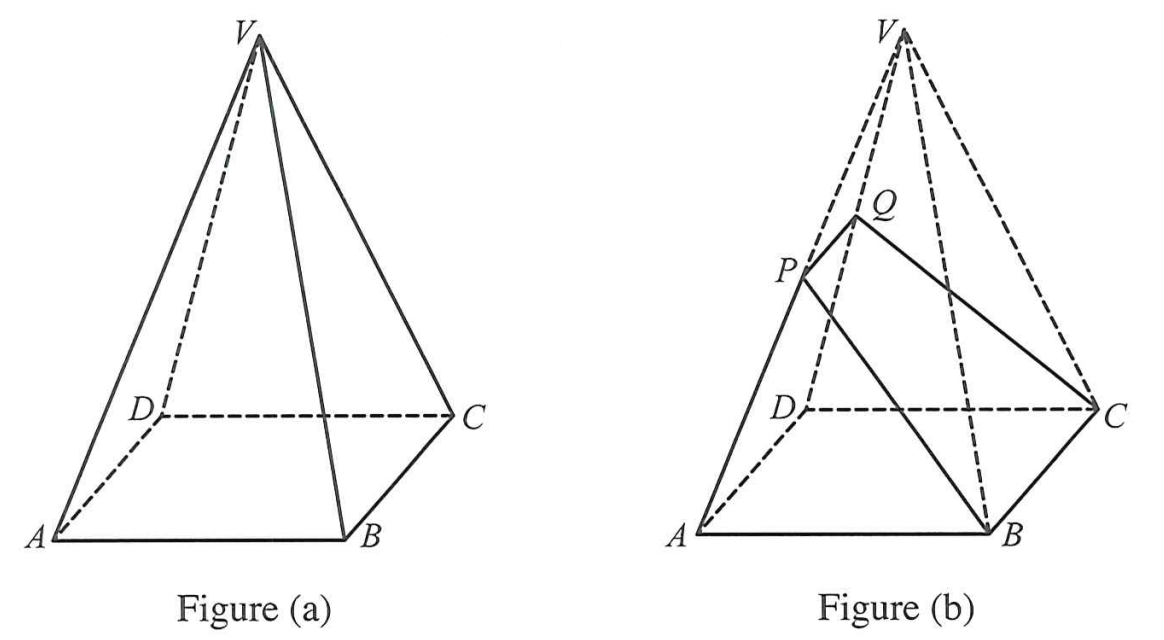
\includegraphics[width=0.75\linewidth]{assets/dijoiqdjoqwjdoqwjdoiqwj.png}\par}
    \begin{parts}
        \part Find the length of AP.\zh{2}
        \part Let a be the angle between the plane PBCQ and the base ABCD.
        \begin{subparts}
            \subpart Find $\alpha$.
            \subpart Let $\beta$ be the angle between PB and the base ABCD. Which one of $\alpha$ and $\beta$ is greater? Explain your answer.
        \end{subparts}\zh{6}
    \end{parts}
    
}
{
    {\par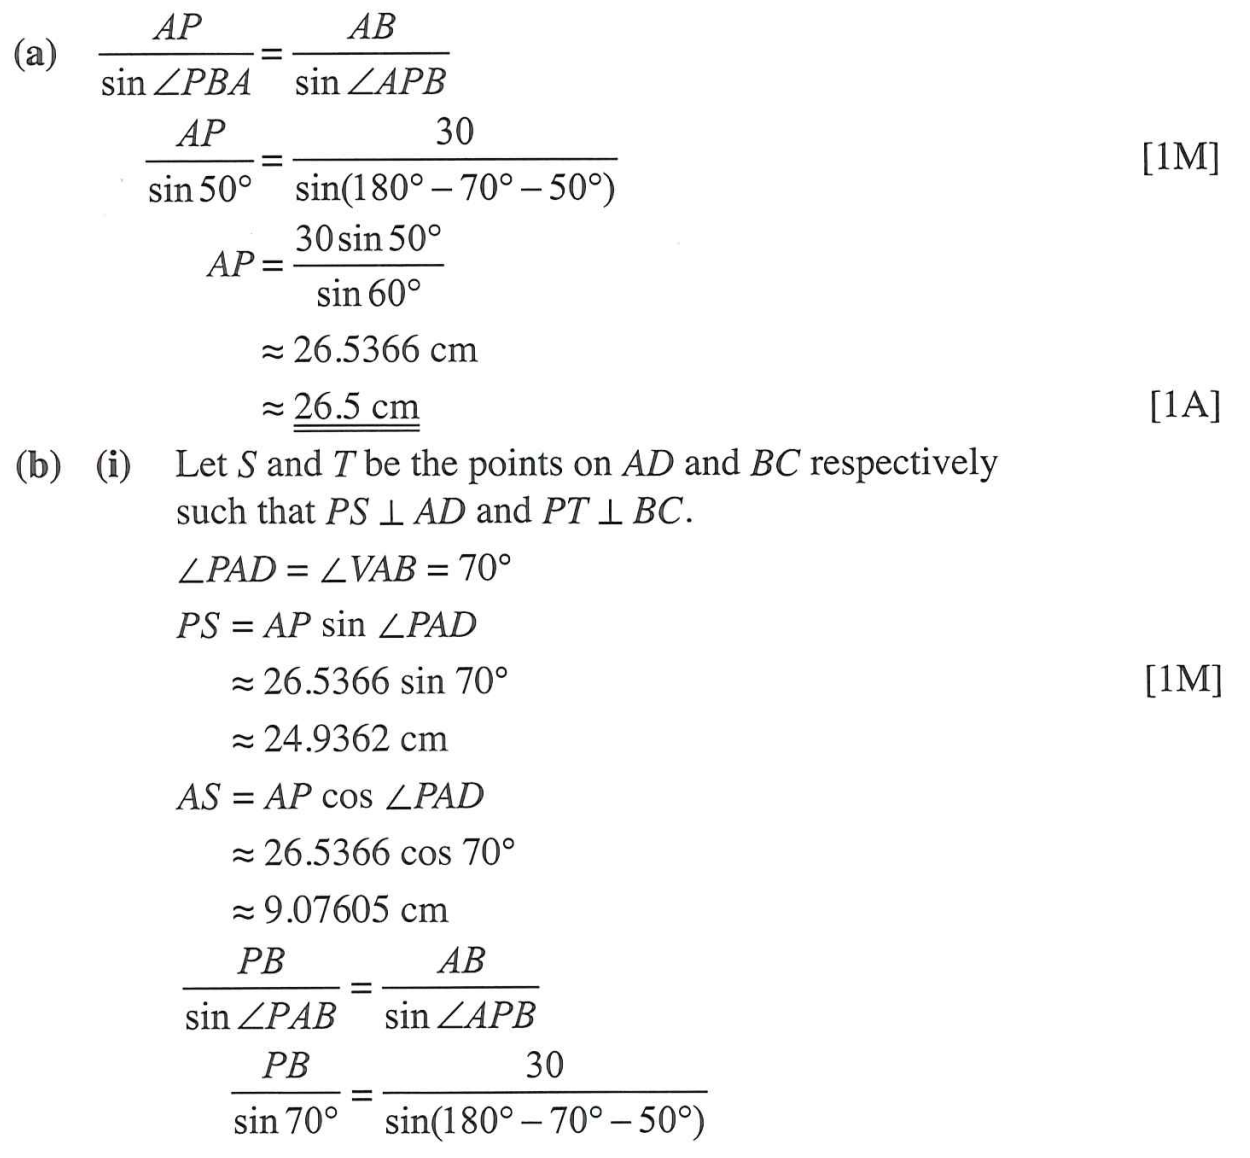
\includegraphics[width=0.75\linewidth]{assets/doijoqwijd.png}\par}
    
    
    {\par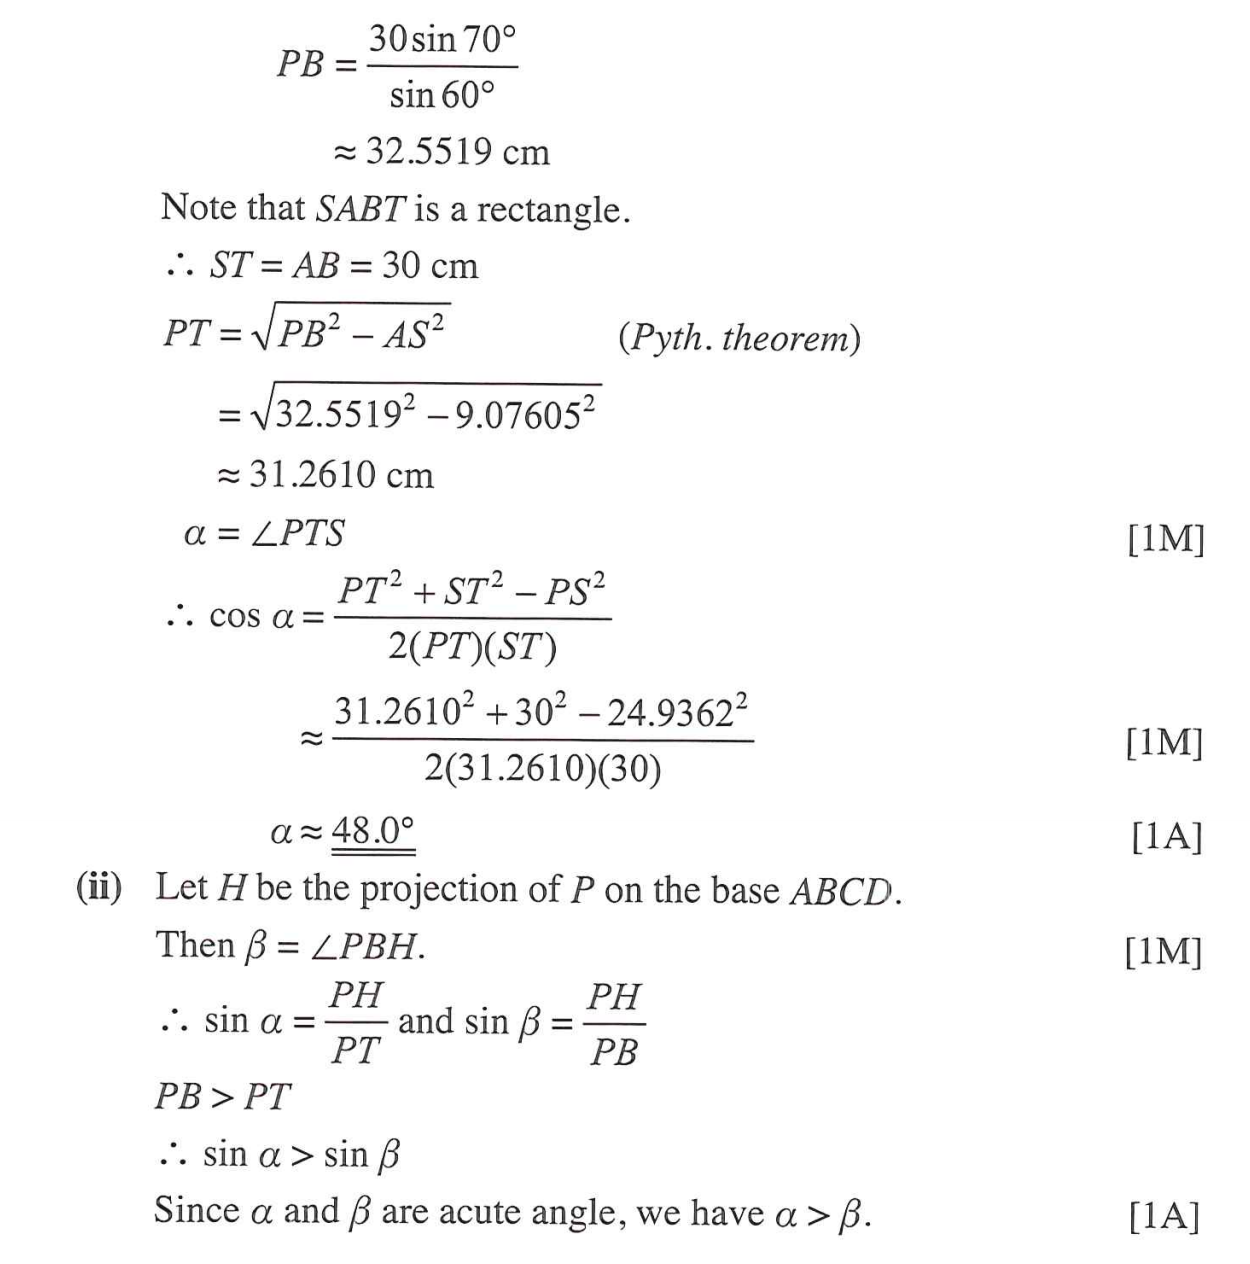
\includegraphics[width=0.75\linewidth]{assets/dwqdjoiqwjdwq1e.png}\par}
    
    
}